\section{Survey Solutions API Client for Stata}
\putimage{pexels-thisisengineering-3861943.jpg}

\vskip16pt
Survey Solutions API client for Stata is a software that facilitates the
control of a Survey Solutions data server from Stata scripts.

\vskip16pt
\subsection{Requirements}

\begin{itemize}
    \item \textbf{Stata 16.0} or newer.
    \item \textbf{Python 3.8} or newer (installed, configured and accessible
    from Stata), additional information here: \newline
    \href{https://www.stata.com/python/pystata/install.html}{https://www.stata.com/python/pystata/install.html}
    \item \textbf{Python modules} (see Dependencies below).
\end{itemize}

\vskip16pt
\subsection{Compatibility with The World Bank Survey Solutions:}
\begin{itemize}
  \item This software has been originally written with Survey Solutions
        v21.01.8 in mind and has been updated for v21.09.5, which is the
        current version at the time of this writing.
  \item Earlier versions may not implement all the functionality that is
        required for it, please update the Survey Solutions server.
  \item Future versions of Survey Solutions may change the behavior of the
        quieries or the formats of responses. If you encounter any
        incompatibility, please check the
        \href{https://docs.mysurvey.solutions/release_notes}{release notes} of Survey Solutions and see if an update is available for this
        API client. Feel free to raise an issue at the
        \href{https://github.com/radyakin/susoapi}{source distribution
        site}, or discuss the problem in the
        \href{https://forum.mysurvey.solutions}{Survey Solutions Users' Forum}.
\end{itemize}

\vskip16pt
\subsection{Installation}
\par
\vskip16pt
\textbf{Where to get:}\par
\begin{itemize}

  \item \textit{Stata}, available for purchase from: \newline
  \href{https://www.stata.com}{https://www.stata.com}

  \item \textit{Python}, available for free download from: \newline
  \href{https://www.python.org/downloads/}{https://www.python.org/downloads/}

  \item \textit{This API client:} in Stata command prompt type: \newline
  \statacmd{ssc install susoapi}

  \item \textit{Survey Solutions server}, available for free download from: \newline
  \href{https://mysurvey.solutions/download}{https://mysurvey.solutions/download}
\end{itemize}

\vskip16pt
\textbf{Checking Python from Stata.}\par
\vskip16pt
When you type the following command in Stata:\par
\vskip16pt
\begin{lstlisting}[style=CommandLineStyle, showlines=true]

python : import sys ; print(sys.version)

\end{lstlisting}
\vskip16pt
you should receive a response indicating Python version. For example: \par
\vskip16pt
\textit{3.8.1 (tags/v3.8.1:1b293b6, Dec 18 2019, 23:11:46) [MSC v.1916 64 bit (AMD64)]}.\par
\vskip16pt
If you are getting an error, then your Python installation is unusable from Stata. Refer to the Stata manual/support on how to install and configure Python for integration with Stata.

% todo: Add list of HTTP codes or a link to such a list.

\vskip16pt
\subsection{Dependencies}
\begin{center}
    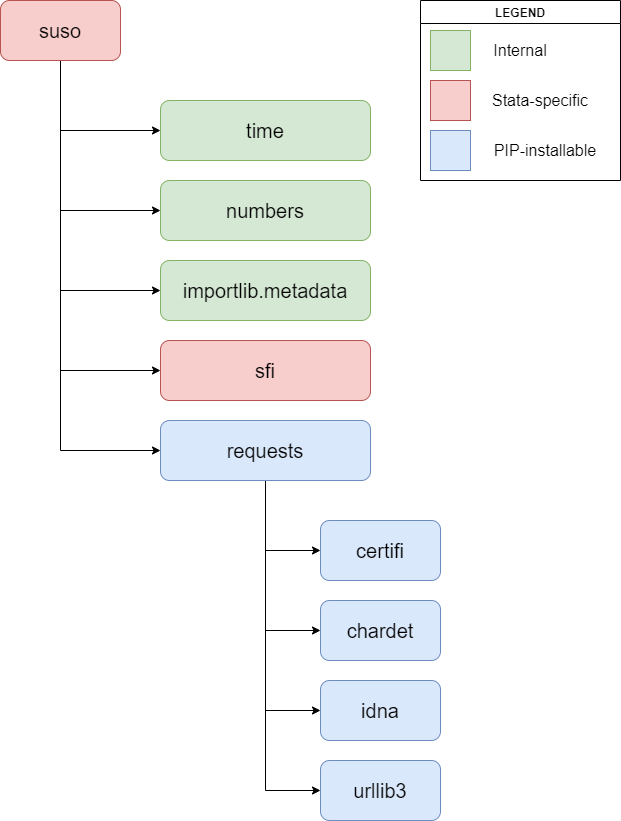
\includegraphics[width=70mm]{images/generated/susoapi-dependencies.png}
\end{center}

Additional module \textbf{requests} needs to be installed with the following
command: \texttt{pip install requests}. (While being installed it pulls its
own dependencies). Additional information here:\newline
\href{https://pypi.org/project/requests/}{https://pypi.org/project/requests/}.

\vskip16pt
\subsection{Create a new API client}
\begin{lstlisting}[style=CommandLineStyle, showlines=true]
.new server username password [workspace]
\end{lstlisting}

\paramsheader
\begin{itemize}

\item \option{server} - URL of the server, for example:
\xmpl{"https://demo.mysurvey.solutions"}

\item \option{username} - name of the API user account, for example:
\xmpl{"WeeklyAPI"}

\item \option{password} - API account password, for example:
\xmpl{"VERY321secret"}

\item \option{workspace} - (optional) workspace name, for example:
\xmpl{"Census"} \newline
If not specified, the default workspace with name \textit{"primary"} is assumed.

\end{itemize}

For example, to set up a client to work with the server \newline
\textit{"https://demo.mysurvey.solutions"}
under the account of user
\textit{"apiuser1"}
with password
\textit{"Secret321Password"}
(not an actual password) and switch to the workspace
\textit{"Jan24"}
we may execute the following Stata code:

\begin{lstlisting}[style=CommandLineStyle, showlines=true]

.demo=.SuSo.new ///
      "https://demo.mysurvey.solutions" ///
      "apiuser1" "Secret321Password" "Jan24"

\end{lstlisting}

After the client is created, we direct all the calls listed in this manual to
the created client object (\option{.demo} in this case) and not to the class
(\option{.SuSo} in this case).

Alternatively, one can use the following syntax:
\begin{lstlisting}[style=CommandLineStyle, showlines=true]
.new :file
\end{lstlisting}

\paramsheader
\begin{itemize}
\item \option{:file} - name of a do-file setting the configuration settings into predefined globals, without an extension (extension *.do is implied) and with mandatory column prepending the name, for example: \textquotedbl\textit{:myserver}\textquotedbl
\end{itemize}

The alternative approach is useful to remove the mentioning of the sensitive information from your main file code into a separate file. If this approach is used, the do-file should set the following globals:
\begin{lstlisting}[style=CommandLineStyle, showlines=true]

    global SUSO_Server="https://...server.name..."
    global SUSO_User="...user.name..."
    global SUSO_Password="...password..."
    global SUSO_Workspace="...workspace.name..."

\end{lstlisting}

These four globals will be substituted in to the corresponding places of the constructor method listed above. Of course one can omit workspace title if not needed, as it is optional.

The file itself may be saved anywhere where Stata searches for files. Check the
documentation for Stata's \option{adopath} command for more information on
this:\newline
\href{https://www.stata.com/manuals/psysdir.pdf}{https://www.stata.com/manuals/psysdir.pdf}.

\subsection{Token-based authentication}
Token-based authentication has been introduced in version 22.02 of Survey Solutions. Users wishing to utilize token-based authentication should follow the same instructions as above, with the following differences:
\begin{itemize}
  \item use specifically \textquotedbl *\textquotedbl \hspace{0.125cm} for the user name;
  \item use the token for the password.
\end{itemize}

\errheader
\begin{itemize}
    \item Error \ecode{5100} is returned if there is an error in establishing a
    secure connection to the server. Typically the code is accompanied with the
    message: \newline
    \textit{``PKIX path building failed: sun.security.provider.certpath.SunCertPathBuilderException: unable to find valid certification path to requested target''}.
\end{itemize}

NB: If you don't specify a workspace, the default workspace is assumed (with
identifier \textit{"primary"}). The client will only be created if the user
with the specified credentials actually has access to this workspace. If not,
make sure you specify an appropriate workspace ID in the constructor.

Workspace may be switched dynamically already after the client has been created,
by assigning:
\begin{lstlisting}[style=CommandLineStyle, showlines=true]
.s.workspace="census"
\end{lstlisting}
